\documentclass[a4paper]{scrartcl}
% Use small margins
\usepackage[left=1.5cm, right=1.5cm, top=1cm, bottom=2cm]{geometry}
\usepackage[unicode,
            pdfencoding=auto,
            pdfinfo={
              Title={Sprawozdanie Wzmacniacz Operacyjny},
              Author={Maciej Mionskowski},
              Subject={Sprawozdanie Wzmacniacz Operacyjny},
              Keywords={},
              Producer={xelatex},
            },
]{hyperref}
\usepackage[T1]{fontenc}
\usepackage{polski}
\usepackage[polish]{babel}
\usepackage[utf8]{inputenc}
\usepackage{upgreek}
\usepackage{array}
\usepackage{amsmath}
\usepackage{mathtools}
\usepackage{caption}
\usepackage{tabularx}
\usepackage{graphicx}
\usepackage{subfig}
\graphicspath{ {images/} }
\renewcommand{\arraystretch}{1.5}

\author{Maciej Mionskowski}
\title{Sprawozdanie 3}
\date{}
\subtitle{Wzmacniacz Operacyjny}
\begin{document}
	{\let\newpage\relax\maketitle}
	{\begin{center}Celem ćwiczenia było zapoznanie się z działaniem, właściwościami i zastosowaniem wzmacniaczy operacyjnych (OpAmp).\end{center}}
	\begin{section}{Wzmacniacz operacyjny w układzie wzmacniacza odwracającego}
		\begin{subsection}{Cel}
			Celem ćwiczenia było dobranie wartości rezystora $R_{2}$ tak aby wzmocnienie $k_{u} = -10 $ i poznanie zasady działania wzmacniacza odwracającego.
		\end{subsection}
		\begin{subsection}{Analiza}
				\begin{figure}[ht]
				\begin{center}
					\label{fig:circuit-1}
					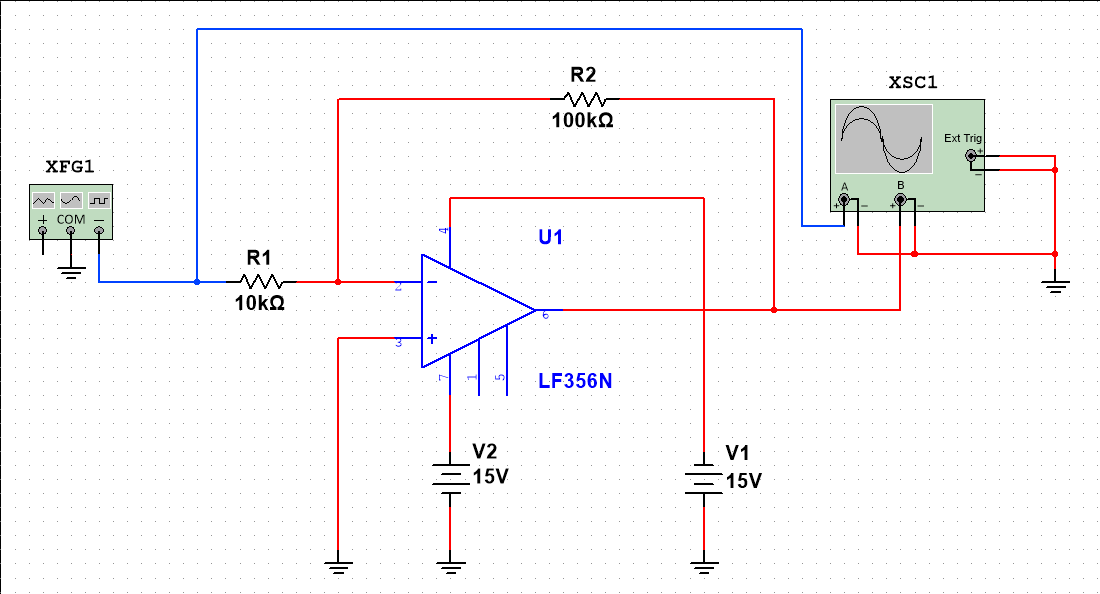
\includegraphics[width=0.8\linewidth]{03-circuit}
					\caption{Schemat ideowy odwracającego wzmacniacza operacyjnego. W obwodzie należało wyznaczyć wartość rezystora $ R_{2} $ }
				\end{center}
				\end{figure}

				\begin{equation*}
					\begin{aligned}
						i_{R_{1}} = \frac{U_{we}}{R_{1}},\; U_{-} = 0V,\; U_{+} = 0V,\; i_{-} = 0A,\; i_{+} = 0A  \\[5pt]
						U_{wy} = -i_{R_{1}}*R_{2}  \\[5pt]
						\frac{U_{wy}}{U_{we}} = \frac{-\frac{U_{we}}{R_{1}}*R_{2}}{U_{we}} = -\frac{R_{2}}{R_{1}} = k_{u} \\[5pt]
						-10k\Omega * -10 = R_{2} \Rightarrow R_{2} = 100k\Omega
					\end{aligned}
				\end{equation*}

				\begin{figure}[ht]
				\begin{center}
					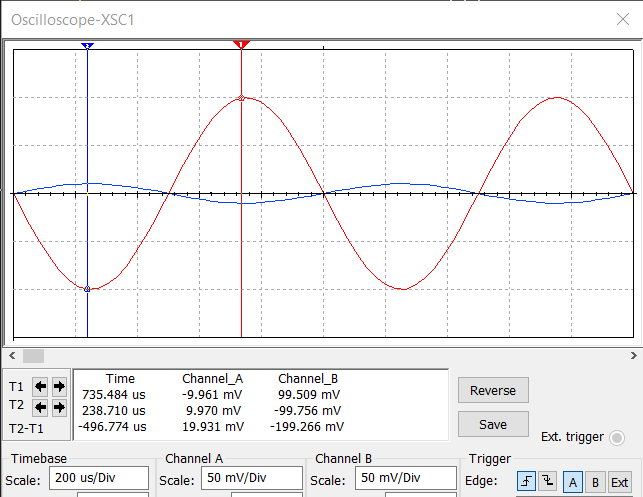
\includegraphics[width=0.6\linewidth]{03-osc}
					\caption{Pomiar napięcia \textit{peak to peak} na oscyloskopie w układzie \ref{fig:circuit-1} celem wyznaczenia rzeczywistego wzmocnienia i potwierdzenia poprawności wykonanych obliczeń.}
				\end{center}
				\end{figure}
				\pagebreak

				Rzeczywiste wzmocnienie układu możemy wyznaczyć wyznaczając stosunek napięć \textit{peak to peak} na oscyloskopie: \\
				\begin{center}
					\begin{math}
					 U_{we} = \vert-9.961\vert + 9.970 = 19.931\quad [mV], \\ 
					 U_{wy} = 99.509 + \vert-99.756\vert = 199.265 \quad [mV],\\
					 k_{u} = \frac{199.265}{19.931} = 9.9977 
					\end{math}
				\end{center}

				\begin{figure}[!ht]
				\begin{center}
					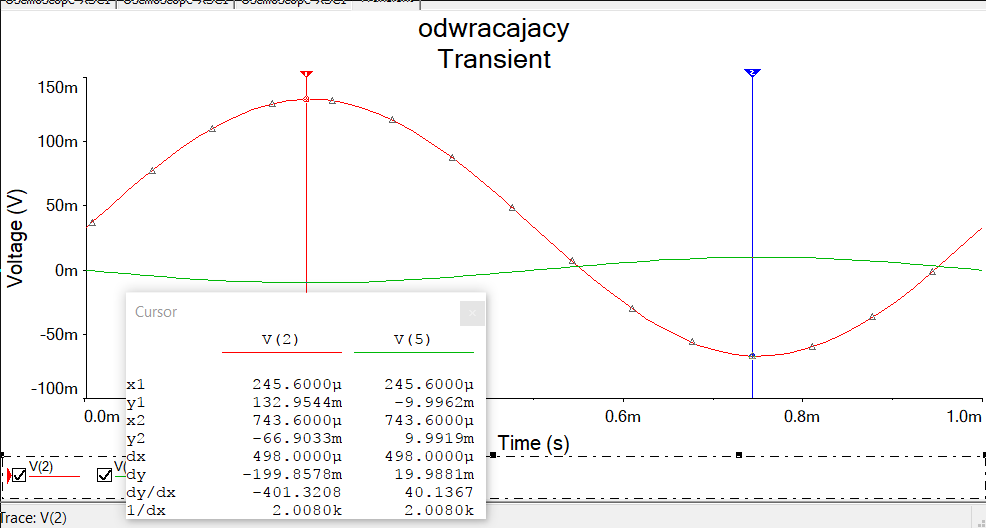
\includegraphics[width=0.7\linewidth,scale=2]{03-peak2peak}
					\caption{Pomiar napięcia \textit{peak to peak} w analizie transient w układzie \ref{fig:circuit-1} celem wyznaczenia rzeczywistego wzmocnienia i potwierdzenia poprawności wykonanych obliczeń.}
					\label{fig:circuit-1-transient}
				\end{center}
				\end{figure}

				Rzeczywiste wzmocnienie układu możemy wyznaczyć wyznaczając stosunek napięć \textit{peak to peak} przy analizie transient: \\
				\begin{center}
					\begin{math}
					 U_{we} = \vert-9.9962\vert + 9.9919 = 19.9881\quad [mV], \\ 
					 U_{wy} = 132.9544 + \vert-66.9033\vert = 199.8577 \quad [mV],\\
					 k_{u} = \frac{199.8577}{19.9881} = 9.9988 
					\end{math}
				\end{center}
		\end{subsection}
		\begin{subsection}{Wniosek}
			Zakładając nieskończoną impedancję wejściową i dążenie wzmacniacza do wyrównania napięć na wejściach możemy dzięki bardzo dobrym rzeczywistym parametrom wzmacniacza wyznaczyć takie wartości rezystorów aby uzyskać dane wzmocnienie. W przypadku powyższego zadania wartość $ R_{2} = 100k\Omega $ jest szukanym oporem, który daje wzmocnienie $ k_{u} = -10 $. Wzmocnienie we wzmacniaczu odwracającym możemy policzyć ze wzoru $-\frac{R_{2}}{R_{1}} = k_{u} $. Drobne rozbieżności rzędu $0.1 \% $ są spowodowane napięciem polaryzującym wzmacniacz i niedoskonałościami programu MultiSim.
		\end{subsection}
	\end{section}

	\begin{section}{Wzmacniacz operacyjny odwracający w układzie sumatora}
		\begin{subsection}{Cel}
			Celem ćwiczenia było zapoznanie z zasadą działania sumatora odwracającego.
		\end{subsection}

		\begin{subsection}{Analiza}
				\begin{figure}[!ht]
				\begin{center}
					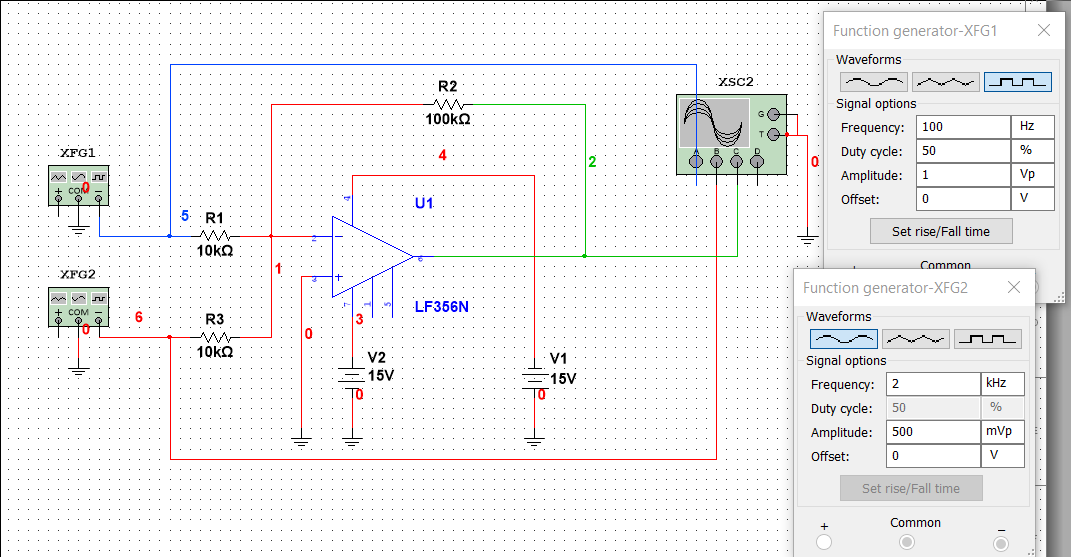
\includegraphics[width=0.7\linewidth,scale=2]{04-circuit-4}
					\caption{Układ wzmacniacza operacyjnego odwracającego w układzie sumatora. Na jedno wejście zapodano sygnał prostokątny a na drugie sinusoidalny.}
					\label{fig:circuit-2-circuit-pre-change}
				\end{center}

				\end{figure}

				\begin{figure}[!ht]
					\begin{center}
						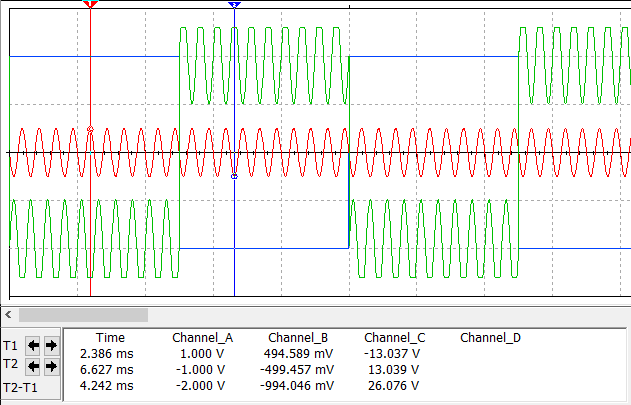
\includegraphics[width=.6\linewidth]{04-osc-4}
						\caption{Sygnał na wyjściu układu sumatora. Można zauważyć, że sygnał sinusoidalny \textit{nakładany} jest na sygnał prostokątny, dodatkowo widać, że sygnał jest odwrócony dzięki zastosowaniu wzmacniacza odwracającego.}
					\end{center}
				\end{figure}
		\end{subsection}
		\begin{subsection}{Wniosek}
			Wzmacniacz operacyjny odwracający w roli sumatora sumuje napięcia zadane na wejściu a następnie odwraca fazę. Dzięki odpowiedniemu dobraniu rezystorów można układ przekształcić w sumator binarny, pozwoli to na późniejsze odseparowanie sygnałów.
		\end{subsection}
	\end{section}

	\begin{section}{Wzmacniacz operacyjny w układzie wzmacniacza nieodwracającego}
		\begin{subsection}{Cel}
			Celem ćwiczenia było dobranie wartości rezystora $R_{2}$ tak aby wzmocnienie $k_{u} = 5 $ i poznanie zasady działania wzmacniacza odwracającego.
		\end{subsection}
		\begin{subsection}{Analiza}
				\begin{figure}[ht]
				\begin{center}
					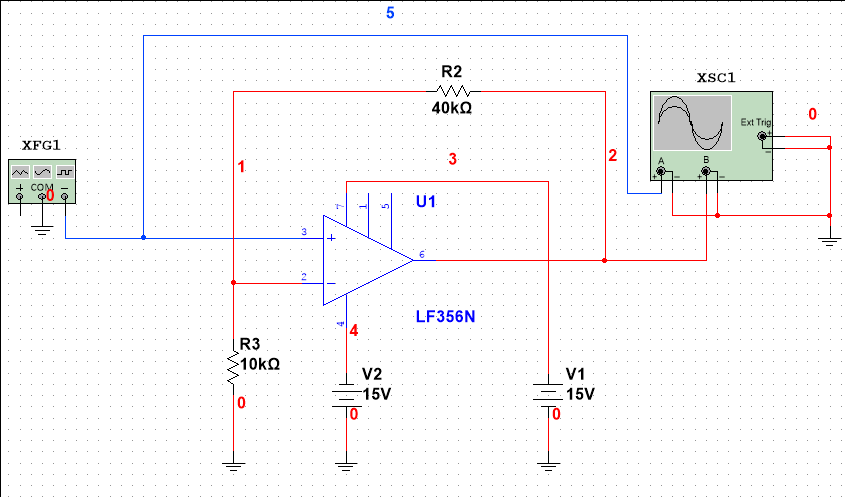
\includegraphics[width=0.7\linewidth]{05-circuit-labels}
					\caption{Schemat ideowy odwracającego wzmacniacza operacyjnego. W obwodzie należało wyznaczyć wartość rezystora $ R_{2} $ }
					\label{fig:circuit-1}
				\end{center}
				\end{figure}
				\begin{center}
					$ i_{R_{3}} &= \frac{U_{we}}{R_{3}},\; U_{-} = U_{we},\; U_{+} = U_{we},\; i_{-} = 0A,\; i_{+} = 0A $ \\[5pt]
					$ U_{R2} = i_{R_{3}}*R_{2} $ \\[5pt]
					$ U_{wy} = U_{R2} + U_{we} $ \\[5pt]
					$ k_{u} = \frac{U_{wy}}{U_{we}} = \frac{U_{R2}}{U_{we}} + 1 $ \\[5pt]
					$ k_{u} = \frac{R_{2}}{R_{3}} + 1 $ \\[5pt]
					$ (k_{u} - 1)*R_{3} = R_{2} $ \\[5pt]

					$ (5 - 1) * 10k\Omega = R_{2} \Rightarrow R_{2} = 40k\Omega $

				\end{center}

				\begin{figure}[ht]
				\begin{center}
					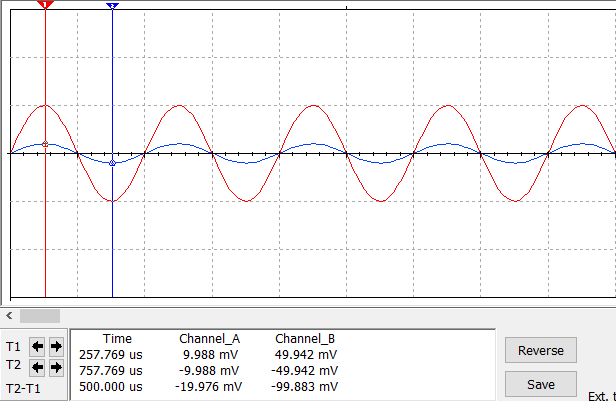
\includegraphics[width=0.7\linewidth]{05-osc}
					\caption{Pomiar napięcia \textit{peak to peak} na oscyloskopie w układzie \ref{fig:circuit-1} celem wyznaczenia rzeczywistego wzmocnienia i potwierdzenia poprawności wykonanych obliczeń.}
				\end{center}
				\end{figure}
				\pagebreak

				Rzeczywiste wzmocnienie układu możemy wyznaczyć wyznaczając stosunek napięć \textit{peak to peak} na oscyloskopie: \\
				\begin{center}
					\begin{math}
					 U_{we} = \vert-9.988\vert + 9.988 = 19.976\quad [mV], \\ 
					 U_{wy} = 49.942 + \vert-49.942\vert = 99.884 \quad [mV],\\
					 k_{u} = \frac{99.884}{19.976} = 5.0002
					\end{math}
				\end{center}

				\begin{figure}[!ht]
				\begin{center}
					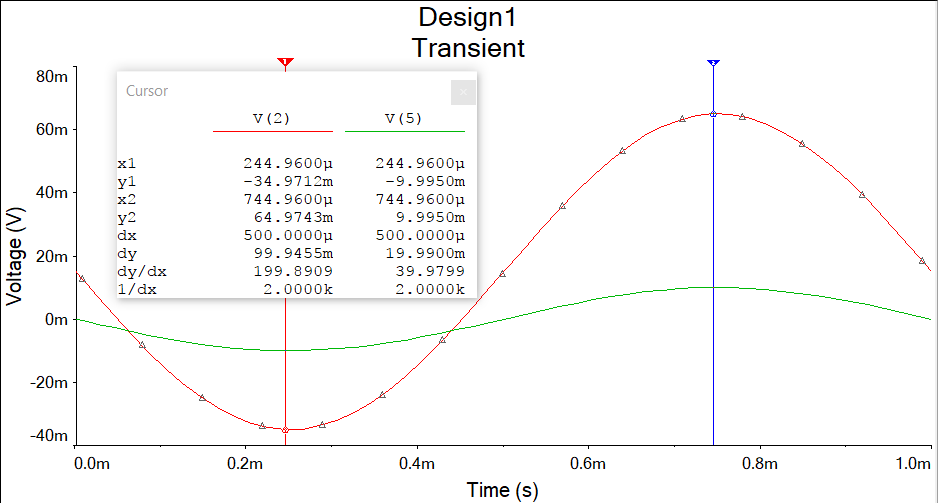
\includegraphics[width=0.7\linewidth,scale=2]{05-transient}
					\caption{Pomiar napięcia \textit{peak to peak} w analizie transient w układzie \ref{fig:circuit-1} celem wyznaczenia rzeczywistego wzmocnienia i potwierdzenia poprawności wykonanych obliczeń.}
				\end{center}
				\end{figure}

				Rzeczywiste wzmocnienie układu możemy wyznaczyć wyznaczając stosunek napięć \textit{peak to peak} przy analizie transient: \\
				\begin{center}
					\begin{math}
					 U_{we} = \vert-9.9950\vert + 9.9950 = 19.99\quad [mV], \\ 
					 U_{wy} = 64.9743 + \vert-34.9712\vert = 99.9455 \quad [mV],\\
					 k_{u} = \frac{99.9455}{19.99} = 4.9997 $
					\end{math}
				\end{center}
		\end{subsection}
		\begin{subsection}{Wniosek}
			Zakładając nieskończoną impedancję wejściową i dążenie wzmacniacza do wyrównania napięć na wejściach możemy dzięki bardzo dobrym rzeczywistym parametrom wzmacniacza wyznaczyć takie wartości rezystorów aby uzyskać dane wzmocnienie. W przypadku powyższego zadania wartość $ R_{2} = 40k\Omega $ jest szukanym oporem, który daje wzmocnienie $ k_{u} = 5 $. Wzmocnienie we wzmacniaczu nieodwracającym możemy policzyć ze wzoru $\frac{R_{2}}{R_{3}} + 1 = k_{u} $. Drobne rozbieżności rzędu $0.1 \% $ są spowodowane napięciem polaryzującym wzmacniacz i niedoskonałościami programu MultiSim.
		\end{subsection}
	\end{section}


	\begin{section}{Wzmacniacz operacyjny w układzie wtórnika napięciowego}
		\begin{subsection}{Cel}
			Celem ćwiczenia było zapoznanie się z zasada działania wtórnika napięciowego.
		\end{subsection}
		\begin{subsection}{Analiza}
				\begin{figure}[ht]
				\begin{center}
					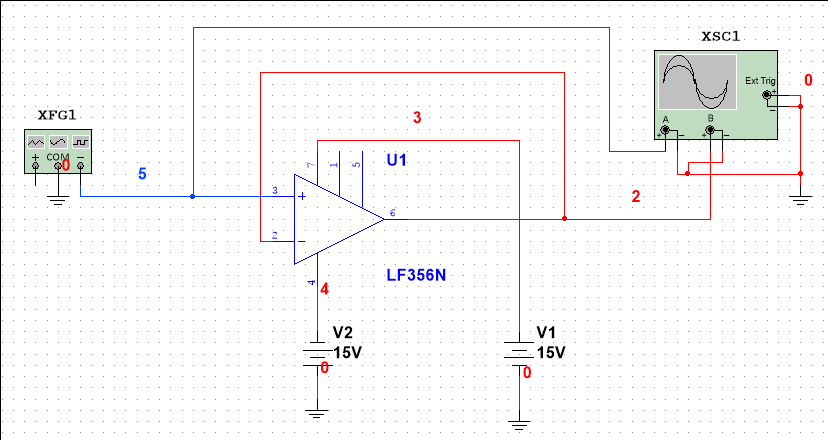
\includegraphics[width=0.65\linewidth]{06-circuit}
					\caption{Schemat układu wzmacniacza operacyjnego w układzie wtórnika napięciowego. Występuje pętla negatywnego sprzężenia zwrotnego.}
				\end{center}
				\end{figure}
				\begin{figure}[!ht]
				\begin{center}
					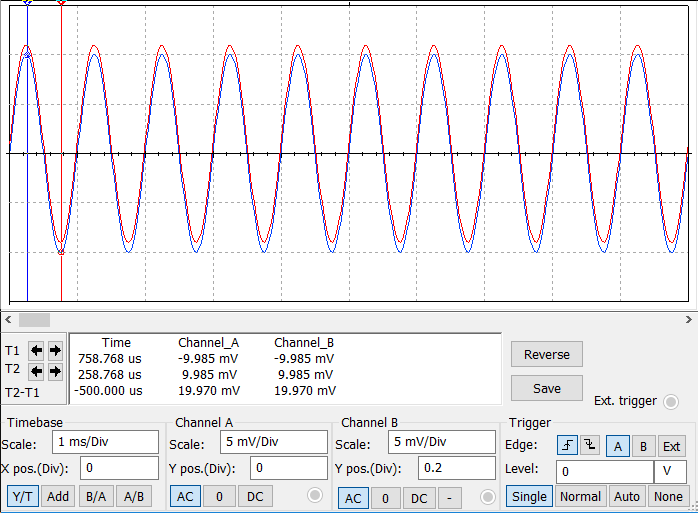
\includegraphics[width=0.6\linewidth]{06-osc}
					\caption{Pomiar napięć wejścia (niebieski) i wyjścia (czerwony). Wykres wyjścia został celowo przesunięty w dół, aby można było rozróżnić przebiegi. Widać, że napięcia się pokrywają.}
				\end{center}
				\end{figure}
				\pagebreak
		\end{subsection}
		\pagebreak
		\begin{subsection}{Wniosek}
			Wzmacniacz operacyjny może być użyty w roli wtórnika napięciowego, pozwala to uzyskać separację obwodów. Na przykład przy dzielnikach napięcia zastosowanie wtórnika pozwala na zachowanie docelowego napięcia nawet przy obciążonym obwodzie. Przy takim samym napięciu wyjścia i wejścia $ k_{u} = 1 $.
		\end{subsection}
	\end{section}
	\begin{section}{Wzmacniacz operacyjny jako integrator}
		\begin{subsection}{Cel}
			Celem ćwiczenia było zapoznanie się z zasadą działania wzmacniacza w roli/układzie integratora - układu całkującego.
		\end{subsection}
		\begin{subsection}{Analiza}
				\begin{figure}[ht]
				\begin{center}
					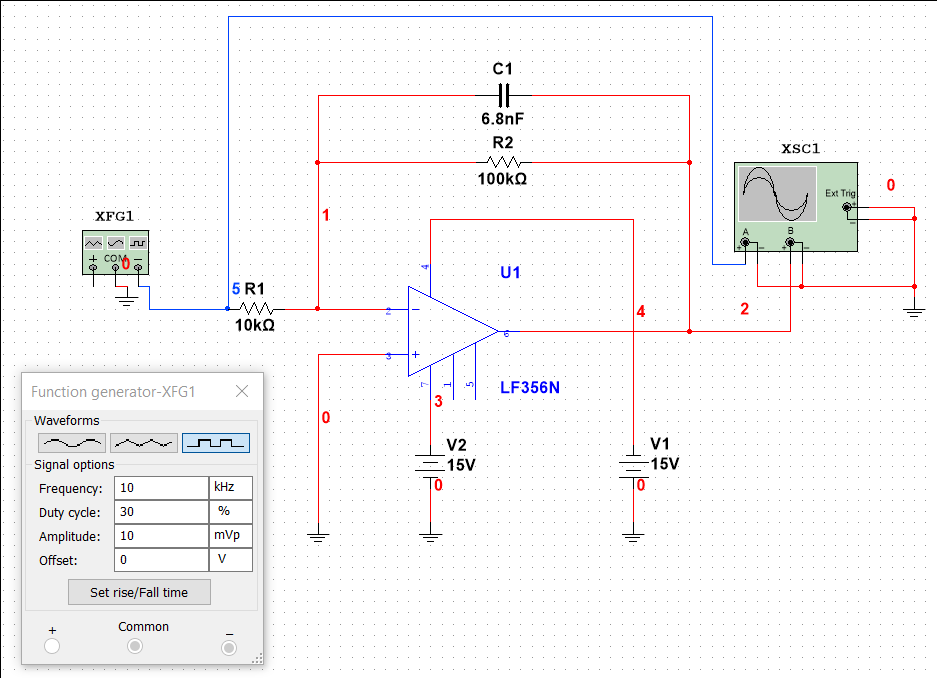
\includegraphics[width=0.5\linewidth]{07-circuit}
					\caption{Wzmacniacz operacyjny w układzie integratora (układ całkujący)}
				\end{center}
				\end{figure}
				\begin{figure}[ht]
				\begin{center}
					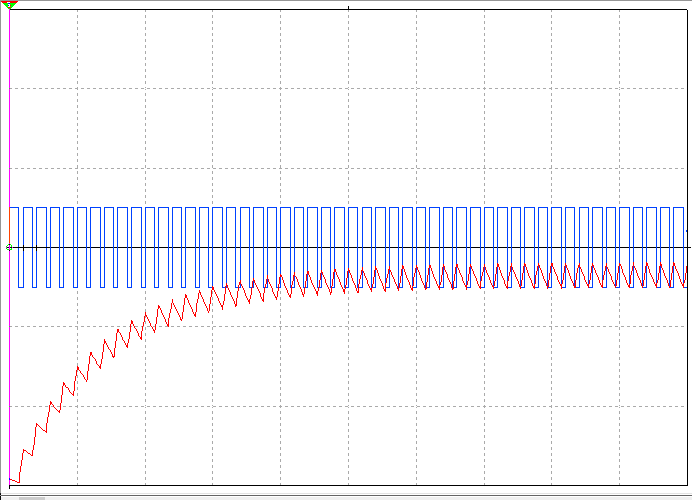
\includegraphics[width=0.5\linewidth]{07-osc}
					\caption{Napięcie na kondensatorze od czasu $ t=0 $. Można zauważyć fazę ładowania się kondensatora.}
					\label{fig:circuit-7-osc}
				\end{center}
				\end{figure}
		\end{subsection}
		\begin{subsection}{Wniosek}
			Wzmacniacz operacyjny może być używany w układach o wielu zastosowaniach matematycznych. Z rysunku \ref{fig:circuit-7-osc} widać jak zmienia się napięcie na kondensatorze wraz ze zmianą napięcia wejściowego. Jako, że zapodany sygnał jest symetryczny względem osi $ OX $ to wartość na kondensatorze jest cykliczna i stabilizuje się. \\
			$ U_{wy} = -\frac{1}{C}\int{i dt}$
		\end{subsection}
	\end{section}
	\begin{section}{Wzmacniacz operacyjny jako aktywny detektor szczytowy}
		\begin{subsection}{Cel}
			Celem doświadczenia było zapoznanie się z zasadą działania układu wzmacniacza operacyjnego w roli detektora szczytowego.
		\end{subsection}
		\begin{subsection}{Analiza}
				\begin{figure}[ht]
				\begin{center}
					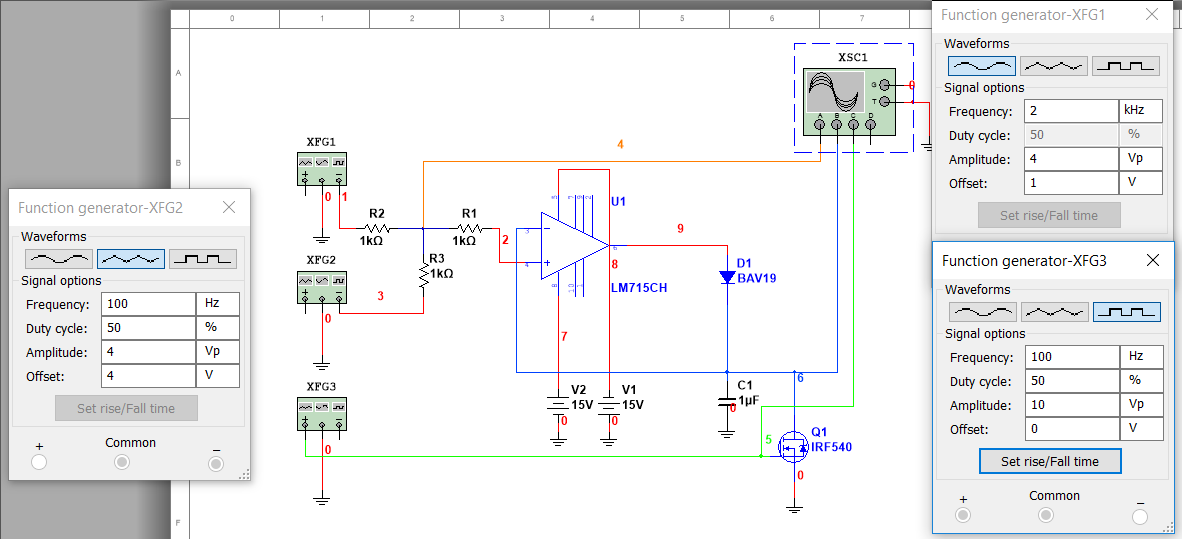
\includegraphics[width=\linewidth]{08-circuit-2}
					\caption{Układ detektora szczytowego ze wzmacniaczem operacyjnym}
					\label{fig:circuit-8}
				\end{center}
				\end{figure}
				\begin{figure}[!ht]
				\begin{center}
					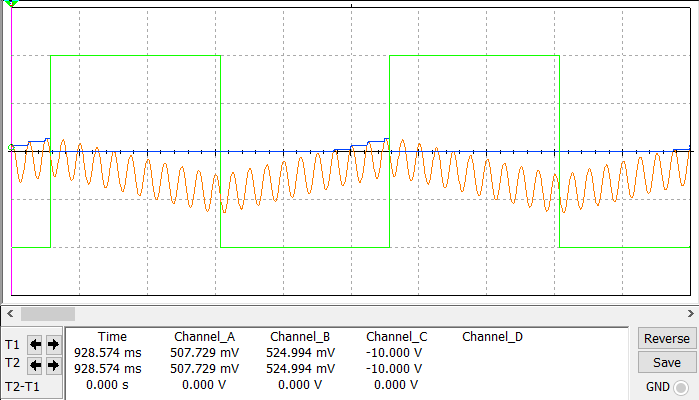
\includegraphics[width=0.6\linewidth]{08-osc-2}
					\caption{Przebieg sygnału wejściowego i wyjściowego w układzie \ref{fig:circuit-8} na oscyloskopie. Sygnał zielony resetuje najwyższy znaleziony szczyt, kanał pomarańczowy reprezentuje napięcie wejściowe, a kanał niebieski ostatni znaleziony szczyt.}
					\label{fig:circuit-8}
				\end{center}
				\end{figure}
		\end{subsection}
		\begin{subsection}{Wniosek}
			Wzmacniacz operacyjny dzięki swoim niemal idealnym parametrom bardzo dobrze sprawia się w roli detektora szczytowego. Wzmacniacz działa tu w roli komparatora i separatora układów. Dioda zapobiega cofnięciu się sygnału.	
		\end{subsection}
	\end{section}
	\clearpage
	\begin{section}{Wzmacniacz operacyjny jako detektor progowy z histerezą}
		\begin{subsection}{Cel}
			Celem doświadczenia było zapoznanie się z zasadą działania wzmacniacza operacyjnego w roli detektora progowego z histerezą
		\end{subsection}
		\begin{subsection}{Analiza}
				\begin{figure}[ht]
				\begin{center}
					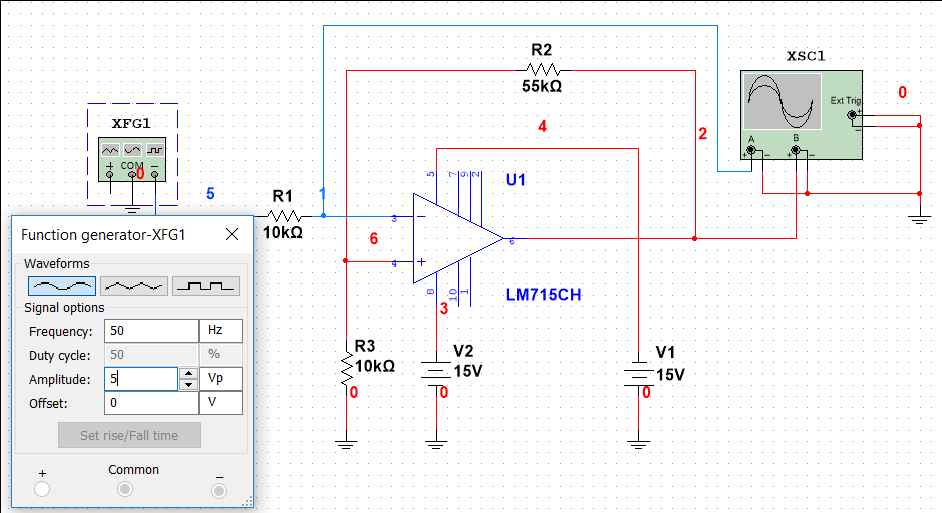
\includegraphics[width=0.8\linewidth]{09-circuit}
					\caption{Układ wzmacniacza operacyjnego w roli detektora progowego z histerezą}
				\end{center}
				\end{figure}
				\begin{center}
				$ U_{p} = \frac{R_{3}}{R_{1}+R_{2}+R_{3}} \Rightarrow R_{2} = 56k\Omega $
				\end{center}
				\begin{figure}[!ht]
				\begin{center}
					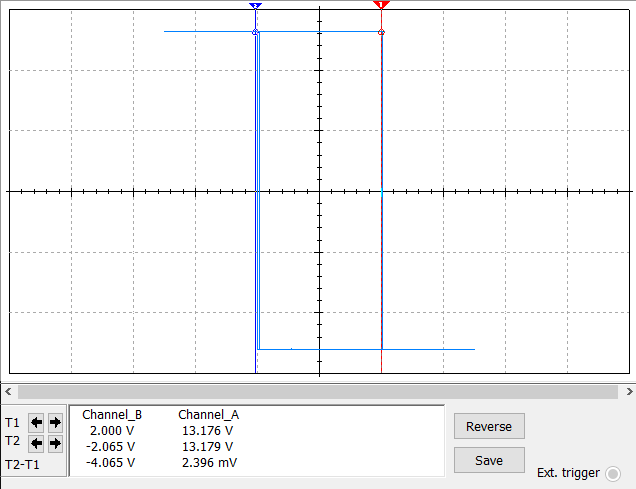
\includegraphics[width=0.7\linewidth]{09-osc}
					\caption{Pętla histerezy, szerokość tej pętli to $ \Delta U_{p} = 4.065V \Rightarrow U_{p1} = 2.0325V, U_{p2} = -2.0325V $}
				\end{center}
				\end{figure}
		\clearpage
				\begin{figure}[!ht]
				\begin{center}
					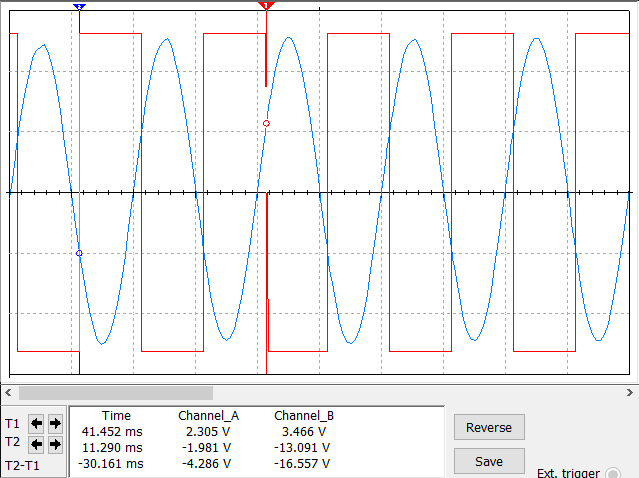
\includegraphics[width=0.7\linewidth]{09-osc-prze}
					\caption{Przebieg sygnału wejściowego i wyjściowego na oscyloskopie. Można zanotować napięcie przełączania $U_{p} = -1.981V$}
				\end{center}
				\end{figure}
		\end{subsection}
		\begin{subsection}{Wniosek}
			Histereza w detektorze szczytowym przydaje się gdy na wejściu mamy sygnał z mocno zaszumionym sygnałem. Szerokość pętli histerezy to różnica między napięciami progowymi.
		\end{subsection}
	\end{section}
	\begin{section}{Wzmacniacz operacyjny w układzie wzmacniacza różnicowego}
		\begin{subsection}{Cel}
		Celem doświadczenia było zapoznanie się z zasadą działania wzmacniacza operacyjnego w roli wzmacniacza różnicowego
		\end{subsection}
		\begin{subsection}{Analiza}
				\begin{figure}[ht]
				\begin{center}
					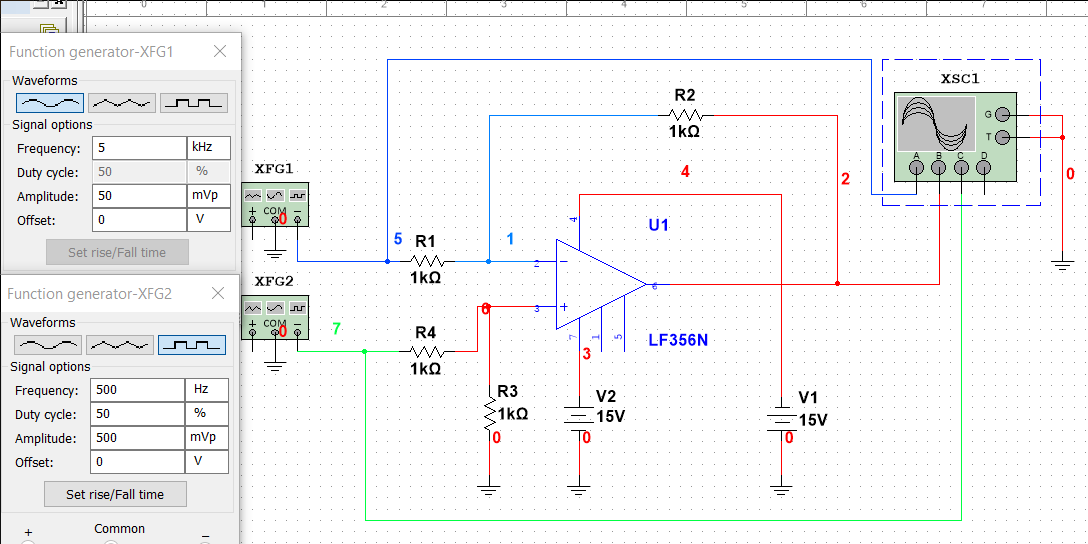
\includegraphics[width=0.7\linewidth]{10-circuit}
					\caption{Układ wzmacniacza operacyjnego w roli wzmacniacza różnicowego}
				\end{center}
				\end{figure}
				\begin{center}
				$ U_{wy} = \frac{R_{2}}{R_{1}}(u_{weA} - u_{weB}) $, gdzie $ R_{2} = R_{3} \wedge R_{1} = R_{4} $
				\end{center}
				\begin{figure}[!ht]
				\begin{center}
					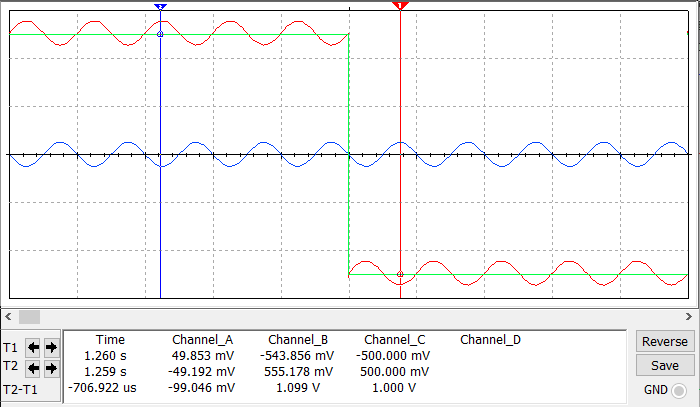
\includegraphics[width=0.7\linewidth]{10-osc}
					\caption{Pomiary napięć w układzie:\\niebieski - $u_{weB} $ \\ zielony - $u_{weA} \\ czerwony - $u_{wy}$, \\ można zaobserwować jak sygnał niebieski jest odejmowany od zielonego.}
				\end{center}
				\end{figure}
		\end{subsection}
		\begin{subsection}{Wniosek}
			Wzmacniacz różnicowy pozwala wyznaczyć różnicę dwóch sygnałów. Jako, że w ćwiczeniu stosunek rezystancji $\frac{R_{1}}{R_{2}} = 1 $ to sygnał nie został wzmocniony. W przeciwieństwie do sumatora przy wzmacniaczu różnicowym sygnał $u_{weB} $ jest odejmowany od $ u_{weA} $
		\end{subsection}
	\end{section}
\end{document}
